\documentclass[12pt]{article}
\usepackage{evolution}

% Guidelines: https://wilsonsociety.org/pubs/wjo/
%TITLE PAGE: place right running head (RRH; shortened title, max 50 characters, capitalize first word and proper nouns only) at top of page, followed by left running head (LRH), author(s) name(s) in regular type: use initials and surname for single author; both surnames connected by ?and? for co-authors; and surname et al. for multi-authors. The running head for Short Communications is RRH: Short Communications.

\begin{document}

%--------------------------------------------------
% TITLE PAGE
%--------------------------------------------------
\noindent\textit{LRH: Igi\'c \& Fenberg} \\
\noindent\textit{RRH: Short Communications: Trainbearer Robbers} \\
\noindent\textit{Version}: \textit{\today}

% Title ideas:
% Neither breaking nor entering: occurrence of secondary nectar robbing in Trainbearers (Lesbia, Trochilidae)

\begin{center}
    %\large{\textbf{Nectar larceny is common in the trainbearers \textit{Lesbia} (Trochilidae)}}
    \large{\textbf{Nectar larceny is common in the trainbearers (\textit{Lesbia}, Trochilidae)}}
\parskip = 0.2in

\normalsize

\noindent 
Boris Igi\'c$^{1}$,
%
and Phillip E.~Fenberg$^{2}$
%
\end{center}
%
\noindent$^{1}$Department of Biological Sciences, University of Illinois at Chicago, Chicago, IL 60607, U.S.A. \\
%
\noindent$^{2}$Ocean and Earth Sciences, National Oceanography Centre Southampton, University of Southampton, Southampton, U.K.\\
%
%


\linenumbers

%--------------------------------------------------
\section*{Abstract}
%--------------------------------------------------

Many hummingbirds engage in floral larceny, a suite of so-called `illegitimate' visits in which birds take nectar without providing pollination services. To the best of our knowledge, we provide the first published report of nectar robbing behavior in trainbearers and analyze the proportion of plant visits categorized by mode of interaction as primary robbing, secondary robbing, theft, and/or pollination.  We then augment our original field observations with a trove of data from citizen science databases and literature to find that ca.~40\% of recorded nectar foraging visits are `illegitimate,' dominated by nectar robbing. We discuss the significance of the findings in the context of recent developments in study of nectar foraging, larceny, and pollination from both avian and plant perspectives.\\
\vfill
% Following the Abstract, include 5 to 7 key words (lowercase except for proper nouns, separated by commas) in alphabetical order that summarize the results of the study.


\noindent \textit{Keywords:} 
nectar robbing, 
floral larceny,
pollination, 
trainbearers, 
hummingbirds, 
feeding behavior

\clearpage

%--------------------------------------------------
%\section*{Introduction} %omit the heading (journal instructions)
%--------------------------------------------------
%
% Floral larceny and its terminology
%
There is a growing list of bird species known to rely on so-called `illegitimate' flower visits, or floral larceny, in which nectar is taken without providing pollination services \citep{irwin2010}.
Floral larceny is correspondingly gaining a broader appreciation as an important factor shaping the ecology and evolution of plant-animal interactions. %lara,ornelas,people who measured plant effects of robbing
Although species such as flower piercers (\textit{Diglossa}, Passeriformes) are widely appreciated to depend on nectar larceny, there are many reports of illegitimate visits by hummingbirds.
Some morphological characteristics of hummingbirds, including bill length and tomial serrations, are thought to be particularly closely associated with nectar larceny \citep{ornelas1994}.

Nearly all plant species that provide nectar and pollen rewards experience larceny, most often from insects and vertebrates, and many defend against it. %cite
The remarkable frequency of illegitimate visits necessitated the development and adoption of a more precise lexicon of larceny \citep{inouye1980}, which attempts to separate it into canonical modes, partly in service of conceptual clarification useful in pursuit of identifying its ecological and evolutionary causes and consequences.
Thus, ``primary nectar robbers'' mechanically create of a hole in flower tissue through which they remove nectar, bypassing the floral opening. 
By contrast, ``secondary nectar robbers'' remove nectar utilizing openings previously fashioned by primary robbers.\footnote{This is stealing without vandalism; the proverbial door was previously broken and now it's a matter of locating any unstolen goods.}
Nearly as a pollinator might, ``nectar thieves'' access nectar through the floral opening. 
Due to a mismatch between flower and thief morphology or behavior, however, pollination does not take place. 
Finally, some plant species are vulnerable to ``base workers,'' visitors that can probe along the base of the flower, between the free petals, and obtain nectar while bypassing both the anthers and/or stigma and the requisite damage or robbing.
These modes of nectar foraging may be difficult to distinguish from each other and/or legitimate visits---pollination---without careful observations and manipulations.
Moreover, they can clearly quantitatively overlap so that, for example, thieving may merely reduce pollination efficiency without eliminating it, or individual birds can engage in a mix of primary and secondary robbing.\footnote{They could also baroquely combine them, for instance, secondarily robbing flowers they primarily robbed, and which they ordinarily legitimately pollinate.}
While many studies report one or more modes of nectar foraging among hummingbirds, we are unaware of any published assessment of their relative importance.
%
%Hummingbirds, tomia, morphology and diets
%
%Set up: Overestimate of primary robbing, points at possibly generally successful defense against primary robbing by hummingbirds, and a possible broader association of chemical defenses and tubular (sympetalous) hummingbird "syndrome" flowers;  Settles Ornelas 1994 vs Rico-Guevara argument by removing many species thought to be primary robbing (without serrated tomia), but allows for serrations to have (dual) functions. See Table 1 in Pelayo2011 for list of many secondary and only one primary robber; list of questions arising in irwin2010.
%
%weller2004: "According to the recent taxonomy (Schuch�mann 1999), Lesbia includes two species, the Black- tailed Trainbearer L. victoriae (Bourcier & Mul�sant, 1846) and the Green-tailed Trainbearer L. nuna (Lesson, 1831)."
% P.S. Weller2004 was knocked down for introducing a third species: see here: http://www.museum.lsu.edu/~Remsen/SACCprop143.htm

% "Here, we" paragraph
Here, we present original observations and a larger meta-analysis of nectar foraging by green- and black-tailed trainbearers (Lesbia nuna and L. victoriae), and discuss their significance in the context of plant-pollinator co-evolution and bill morphology. The original observations took place in and around Ollantaytambo, Peru, on \textit{Brugmansia sanguinea}, \textit{Fuchsia boliviensis}, and \textit{Passiflora tripartita}.  We document the proportion of pollination, theft, and primary- and secondary-robbing visits to flowers, by leveraging images from citizen-science databases eBird, iNaturalist, and other photographed/reported occurrences in the literature. Our highly preliminary analyses find that floral larceny is surprisingly common, at least ca. 40\%, and that secondary robbing may be more common among hummingbirds than is generally appreciated, further complicating the proposed association between tomial serrations and mode of nectar foraging. %many illegitimate visits are on flowers pollinated by Ensifera, but some unexpected ones, too! "further complicating" should be later explained in terms of other hypotheses for presence of tomial serrations, as well as the implication of common secondary robbing.
\\

%--------------------------------------------------
\section*{Materials and Methods}
%--------------------------------------------------

\subsection*{Site description}

On January 14th, 2019, we recorded and photographed a male green-tailed trainbearer, Lesbia nuna (Lesson, 1832), which nectar-robbed several flowers of \textit{Fuchsia boliviensis} (Onagraceae) in Ollantaytambo, Peru ($13^{\circ}$15$'$44$''$S, $72^{\circ}$16$'$14$''$W), and then followed the same individual on a 50m foraging bout, while it nectar-robbed flowers of \textit{Brugmansia sanguinea} (Solanaceae)---a species with spectacular ca. 30cm-long tubular crimson-to-yellow flowers---and then legitimately visiting \textit{Salvia leucantha} (Lamiaceae). Both rusty and black-throated flowerpiercer (\textit{Diglossa sittoides} and \textit{D. brunneiventris}) occur at relatively high densities in the area (B.I. and P.B.F., unpub. data), are known to pierce both \textit{Fuchsia} and \textit{Brugmansia} species, and may have been responsible for the previously made calyx and petal hole at the base of \textit{B. sanguinea} flower.

\subsection*{Literature searches}

We examined the literature and internet resources to accumulate a database of additional instances of nectar collecting visits by \textit{Lesbia} species. 
First, we used internet and Google Scholar keyword searches of the existing scientific literature (e.g. `Datura' or `Brugmansia' and `Lesbia' or `trainbearer'; `Lesbia' and  `diet'). 
Documentation of any details on foraging ecology of the trainbearers is sparse. 
We found two references hinting at illegitimate flower visits by trainbearers. \citet[p.15]{gould1861} cited in \citet{ornelas1994}, contains a passing reference to piercing of a \textit{Brugmansia sp.} flower by a \textit{Lesbia sp.}, but the visit was inferred as insect predation, not nectar robbing, as later re-framed by \citet{ornelas1994}, and neither the species nor locations were identified. 
In a paper documenting secondary robbing behavior in cinereus conebills, \citet{vogt2006} mentions unpublished observations of secondary nectar robbing by a trainbearer species on a species of \textit{Fuschia}.  
Our literature search and two substantial meta-analyses \citep{ornelas1994,irwin2010} did not retrieve any other references to illegitimate visits by these species. 
Additionally, although we could find no papers documenting their foraging ecology in any detail, gut contents of a single individual examined did include arthropods \citep{remsen1986}. 
Therefore, as generally holds for hummingbirds, the trainbearers' diet minimally contains arthropods and nectar. 
The mode of nectar foraging is, however, unclear. 

\subsection*{Foraging data collection and scoring procedures}

Consequently, we examined all identified species records for the Genus \textit{Lesbia} in two public databases---iNaturalist \citep{inaturalist} and eBird \citep{ebird}. 
For all resulting records, we applied the same methodology. 
Images without any flowers were discarded, as were those in which birds were simply perched or flying near a flower.
We then closely examined the remaining images, in which birds were hovering in close proximity (about a body length) to flowers, and facing them. 
For that subset, we extracted the location, date, and comment metadata. 
We scored individual sex (`m',`f', or unknown), re-visited distinguishing marks and confidence of species identification (scoring specific epithets as `nuna', `victoriae', or `sp.'), estimated the mode of interaction (primary nectar-robbing, secondary nectar-robbing, thieving, pollination, or unknown), as well as our confidence in the estimate of the mode of interaction (Low vs. High). 
Finally, with the help of several colleagues, we identified the visited plant species. 

Often, modes of interaction are unclear and we combined terms for the most accurate characterization of interaction. 
For example, primary vs. secondary nectar robbing and pollination vs. thieving are generally hard to distinguish, so we simply combined the likely interactions. 
This enables us to conservatively summarize modes of interactions as approximate ranges, without making unnecessary assumptions.
While identification of trainbearers is relatively easy, assignment of the species epithet can be difficult, on account of great amount of geographic variation and possible existence of undescribed species \citep{weller2004}. %figure out how to cite this: http://www.museum.lsu.edu/~Remsen/SACCprop143.htm
Therefore, while we recorded the species-level data, we often found identifications to be implausible or uncertain, and we jointly present the feeding habits for all \textit{Lesbia}. %until the taxonomy is clearer

\subsection*{Bill morphology}

Short-billed hummingbirds and those with serrated tomia are thought to be more likely to nectar-rob, especially flowers with long corolla tubes, co-adapted with long-billed hummingbirds \citep{lara2001}. 
We did not find a reference to presence/absence of serrated tomia in trainbearers, so we scored this trait in 13 specimens at the Field Museum of Natural History.
We used a dissecting microscope to visualize and score this trait on the available collections (12 males and one female), as well as measure their bill lengths. 
%(accessions: FMNH46385, FMNH222248, FMNH222249, FMNH222250, FMNH222251, FMNH222252, FMNH222254, FMNH222255, FMNH299096, FMNH208193, FMNH299095, FMNH208194, \& FMNH46392).
% We could not score the serration phenotype in one specimen (male, FMNH222253), as its bill was inconveniently glued together.
%Tomial serrations are sometimes difficult to score on dried specimens, so we first examined specimens known to display serrations (e.g., \textit{Colibri coruscans}, specimen FMNH179303). 

All metadata, image locations, and scored data used in our analyses are available online in Supplemental Materials.
\\

%--------------------------------------------------
\section*{Results}
%--------------------------------------------------

% fixme: need to state our own observations clearly.
In our field observations, we recorded a single adult male foraging bout, during which this individual visited flowers of three plant species. Approximately ten flowers of \textit{Fuchsia boliviensis} were robbed (unclear if primary or secondary robbing took place) as well as two flowers of \textit{Brugmansia sanguinea}, while five flowers of \textit{Salvia boliviensis} were apparently legitimately visited (ruling out or confirming effected pollination requires controlled experiments). 
Photographs collected in the course of observations were deposited in a single record on iNaturalist (\href{https://www.inaturalist.org/observations/37206000}{https://www.inaturalist.org/observations/37206000}; \citealt{inaturalist}).

In addition, we collected and examined a total of 180 individuals' floral visits on 42 flowering plant genera \cref{figure:fig1}. %fixme (re-count and fix "42" after identifying all plants)
The mode of interaction for 135 visits could be assigned with some confidence, while the mode of visit interaction for 45 visits is unknown, often because birds were hovering in the vicinity of a flower, immediately before or after nectaring.
The most common recorded mode was `pollination/thieving'  (46 visits), a category that we conservatively scored as vague because it was nearly impossible to disentagle those modes in many cases, without functional study (bagging and marking flowers).
Our impression, however, is that the majority of these visits plausibly resulted in pollen transfer.
The second most common mode was combined `nectar robbing' (primary and secondary robbing; 41 visits) indicating that an individual fed through a pierced hole in the side of the corolla.
It was followed by `pollination' (36 visits), which indicated a fairly clear legitimate interaction, `secondary nectar robbing' (10 visits), and thieving (2 visits). 
Although we could not confidently assign any visits to the `primary robbing' mode, this is almost certainly only due to the limitations of our approaches.

An examination of 13 specimens of \textit{Lesbia nuna} revealed no evidence of serrations. The imbalance of sex ratio (12 males) is not likely to be important in this instance because serrations are more likely to be present in males \citep{}. %FIXME
The mean bill length for males was $16.89 \pm 0.47$ mm. 
The female's bill measured $17.38$ mm.


%--------------------------------------------------
\section*{Discussion}
%--------------------------------------------------

%
% Some kind of nectar robbing is common
%
%Nearly all relevant reports of nectar foraging simply provide presence (or imply absence) of nectar robbing, and do not provide an estimate of the proportion of visits dedicated to illegitimate visits. A few existing studies indicate that, for the species surveyed, the frequency of nectar robbing at the individual-plant level is highly variable, ranging between 8.5-57.6\%. (arizmendi2001) and up to 92% of all flowers in Salvia mexicana (Arizmendi1996).
%
%Feinsinger 1987: "Anthropogenically generated disturbance mosaics may promote the spread of species whose reproductive traits evolved under very different circumstances from mosaics generated by natural disturbances." Both species of trainbearers occupy heavily degraded habitats, and many observations are in disturbed, populated areas. 
%
% Stiles 1995 the Condor: More than half of all foraging efforts (both nectaring and predation) involve hunting for arthropods. Nectaring is actually the less-frequent activity.
%
% Floral larceny is stereotypically committed on plants that have close co-evolutionary relationships with other animal species, such as sicklebill hummingbirds and sickle-shaped flowers of Centropogon sp.
% Some morphological characteristics of hummingbirds, including bill length and tomial serrations are thought to be particularly closely associated with nectar larceny \citep{ornelas1994}.
%
While short-billed hummingbirds stereotypically rob nectar from long sympetalous tubular flowers, competing with legitimate long-billed legitimate visitors, like sword-billed hummingbirds (Ensifera ensifera), observational data presents a slightly more textured picture, with remarkable displays of opportunism. For example, we found a number of documented visits by Lesbia sp. to the composite flowers of Asteraceae (daisy family), as well as the remarkable images of apparent nectar robbing of Brugmansia sanguinea by sword-bills.  %fixme check ID on lesbia

%
% Secondary nectar robbing is common and, at least in this species, primary nectar robbing may be rare
%
Our findings show that secondary nectar robbing is relatively common, comprising between 7.4\% and 37.8\% of the visits. If it is true that, on the whole, primary robbing allows access to previously unvisited, relatively nectar-rich flowers, then secondary robbing should generally be disadvantageous \citep{irwin2010}.  In this context, our relatively high observed frequency may appear somewhat paradoxical, and more likely, one or more of our underlying assumptions are flawed.  Specifically, we can imagine that, for example, if they are faced with limited supply of resources that are easily legitimately exploited, trainbearers likely respond by robbing or thieving from inferior resources, a situation that may be exacerbated by territoriality. 
%
% THREE-WAY CONTINGENCY TABLE (counts of LarcenyYES/LarcenyNO, M/F, nuna/victoriae)
%
%
%nice stats page: https://dev.stat.vmhost.psu.edu/stat504/book/export/html/720
%facetting: http://haleyjeppson.github.io/ggmosaic/articles/ggmosaic.html
%
% FIXME: Why we think secondary robbing is at the high end of that range?: Diglossa common in the area(s) across Lesbia range (unpub/supp info), observations likely biased against secondary robbing--rare examination prior to visit?


%
% How this jives with Ornelas 1994 and Rico-Guevarra 2019
%
% rico-guevarra2019: "Regarding the flower-piercing hypothesis (Ornelas 1994), this idea was proposed before it was taken into consider- ation that the expression of the tomial serrations is sexually dimorphic (e.g., Rico-Guevara 2014). Consequently, one would expect differences in nec- tar robbing between the sexes. However, males of serrated species have not been reported to pierce more than females, and the reports of nectar rob- bing are not skewed toward hummingbird species with serrated tomia (Robert Colwell personal com- munication). Additionally, hummingbird species that are considered specialized piercers (e.g., Wedge-billed Hummingbird [Schistes geoffroyi], Purple-crowned fairy [Heliothryx barroti]) do not present these sexually dimorphic serrations (Rico- Guevara and Rubega 2017). A thorough discussion of these and other alternative hypotheses for the evolution of serrated tomia in hummingbirds will be provided elsewhere (Gary Stiles personal communication)."

% Complicates ornelas1994 and naysaying: if robbing, and especially, secondary robbing is more common than previously thought, and serrations are more common in males these facts can interact with male territoriality---males inflexibly feed and may need to extract all the resources, despite some costs; moreover it's possible that male-male interactions and robbing are exaptively interacting.

The presence of serrated tomia on the bills of some hummingbird species may represent an adaptation shaped by nectar robbing \citep{ornelas1994}. 
It remains unclear, however, if the presence of serrated tomia affects nectar robbing ability and efficiency. 
Recent studies suggest that the presence of serrations is sexually dimorphic, with greater or exclusive expression in males, and that this feature could instead be shaped by a role in plumage preening or fighting, especially male territorial defense \citep{rico-guevara2019}. Although additional field studies of nectar robbing and examination of bill morphologies for the presence of serrate tomia are needed to clarify their role, our data provide some insight and a possible resolution of apparent contradictions.
% If secondary nectar robbing is more common than previously thought, the number of paired serration+primary robbing observations would be low and more difficult to detect. 
% Moreover, neither sexual dimorphism nor the proposed role in defense precludes simultaneous or exaptive function of serrated tomia in piercing, which makes the collection of weight of evidence in exclusive support of either hypothesis difficult.
% It is worth noting


%
% Consequences for ecology and evolution of plant-animal interaction
%
%
% discourages animal specialization (gonzalez and loiselle 2016), discourages plant specialization as well as shortening corollas (lara and ornelas 2001), and affects plant defenses; emphasize that it's not only tube length (cite) and shape (boehm/centropogon), but also secondary metabolites.
%
Both modes of larceny are also likely to cause both plastic and evolutionary responses from flowering plants, including variation in proportion and/or time-dependence of nectar release, and placement of secondary metabolites. Interestingly, a number of plant species visited by trainbearers, including members of the nightshade family (Solanaceae), produce alkaloids broadly toxic to vertebrates. For example, \textit{Brugmansia} species can temporarily incapacitate (much larger) juvenile humans by skin contact alone \citep{andreola2008}. 
Perhaps not coincidentally, a great number and quantity of alkaloids are produced by species of \textit{Brugmansia} and \textit{Nicotiana}, and tissues at the base of flowers (calyx) contain some of the highest concentrations of such compounds \citep{saitoh1985, alves2007}. 


%
% Concluding paragraph
%
Our observations and analyses point to additional needed work on systematics and ecology of \textit{Lesbia}, especially their unsettled taxonomy, feeding ecology and energy budgets.  %work into taxonomic confusion: http://www.museum.lsu.edu/~Remsen/SACCprop143.htm
More broadly, we sorely lack observational data to establish the relative frequencies of nectar feeding modes and detailed manipulative field study to obtain direct evidence for nectar feeding dynamics across all hummingbirds and other nectar-feeding birds \citep{irwin2010}.
Similarly, a better understanding of plant-side effects and responses, including pollination efficiency, the distribution of visitor interactions \citep{arizmendi2001}, as well as plant incentives and defenses, may help us better explain the dynamics in the co-evolutionary game between flowers and their visitors.

%--------------------------------------------------
\section{Acknowledgements}
%--------------------------------------------------

We thank iNaturalist and eBird projects, and all contributing citizen naturalists whose images and data enabled us to conduct this study. We thank Diego Emerson Torres (\href{https://ebird.org/profile/NzU3NjIy}{https://ebird.org/profile/NzU3NjIy}) for permission to use the image in Figure 1.
This work was supported in part by the National Science Foundation NSF DEB-1655692.

%--------------------------------------------------
% References
%--------------------------------------------------
\clearpage

\setstretch{1}
\bibliography{nectar-robbing}
\bibliographystyle{evolution}
\setstretch{\stretchby}

%--------------------------------------------------
% Figures
%--------------------------------------------------

%TABLES & FIGURES in-text references to figures and tables should be parenthetical to the text (i.e., cited only in parentheses to support text) Use a consistent font and style throughout (e.g., 12-pt font, Times New Roman is preferred). Do not use boldface font for figure keys and axis labels. Capitalize first word of figure keys and axis labels; all other words are lower case except proper nouns.

\begin{figure}
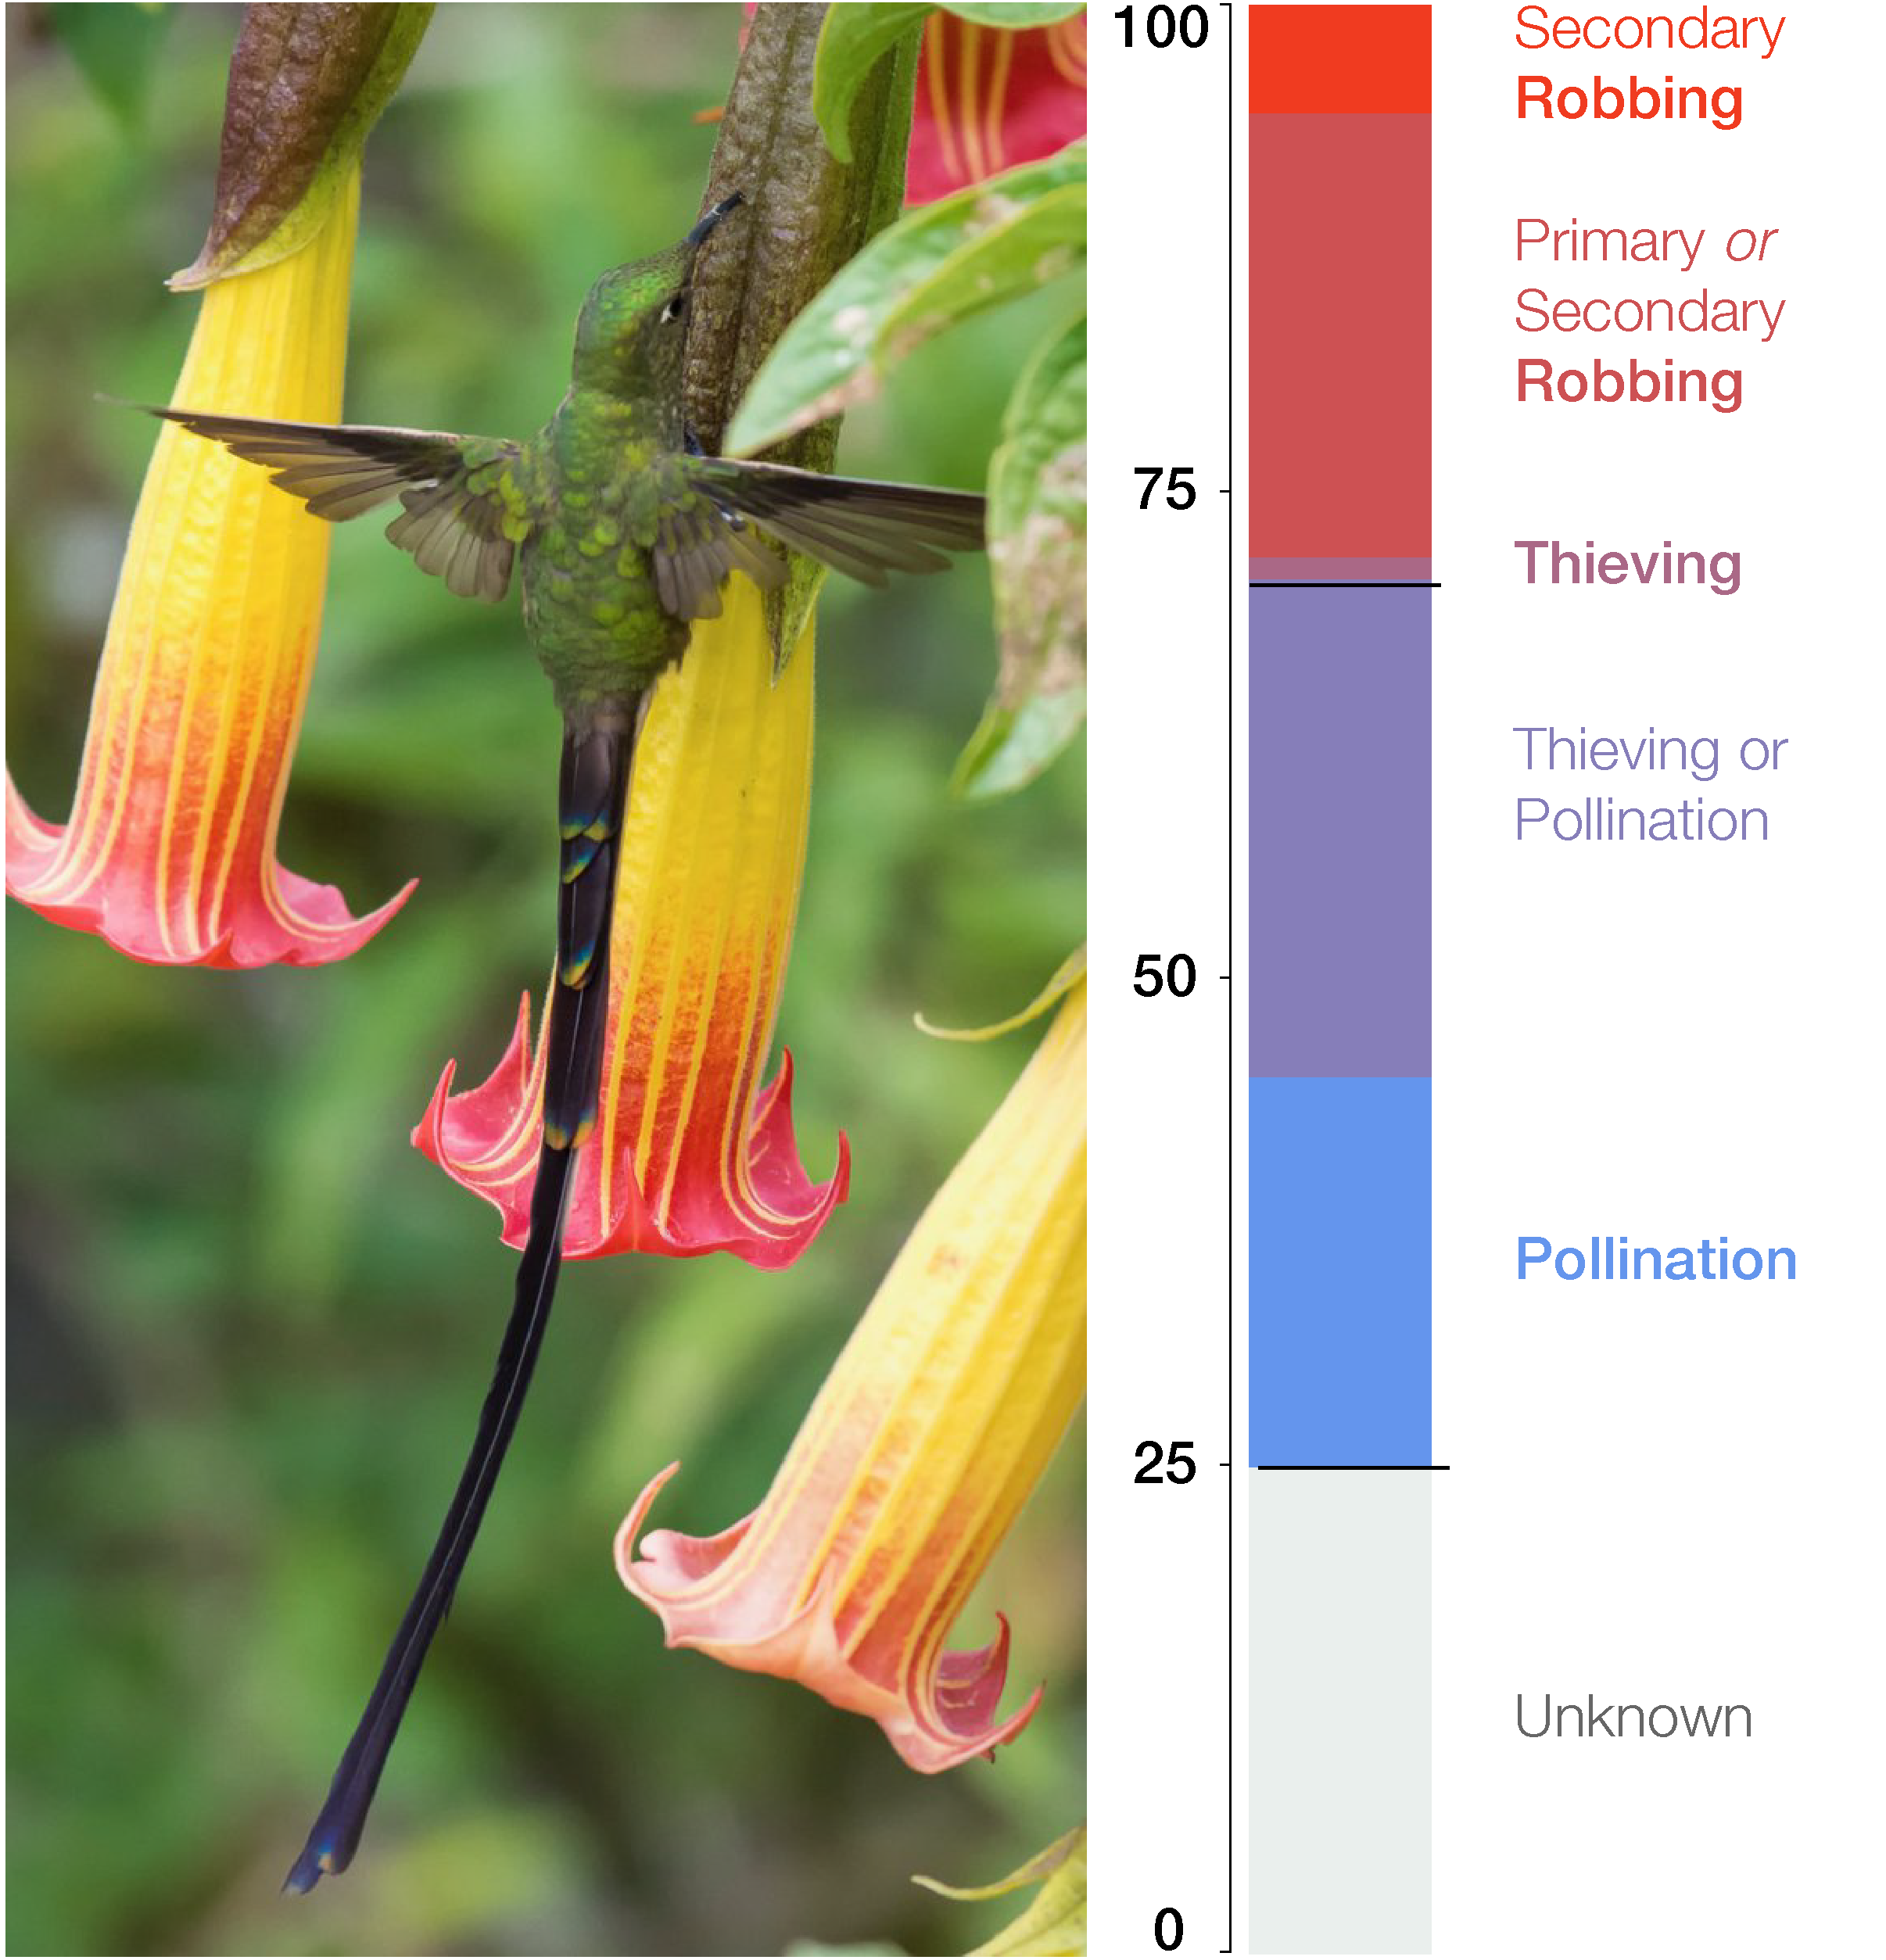
\includegraphics[width=1\textwidth]{fig1/marauding_lesbias_fig_1b.pdf}
\caption{A nectar robbing visit by a black-tailed trainbearer \textit{Lesbia victoriae} on \textit{Brugmansia sanguinea}, whose flower was previously pierced by a species of \textit{Diglossa} (Photo by Diego Emerson Torres; used with generous permission of author). Right panel: A bar plot illustrating the relative visit mode frequencies of \textit{Lesbia} species (n=180).}
\label{figure:fig1}
\end{figure}

\pagebreak

\begin{suppfigure}
\begin{center}
\includegraphics[width=0.5\textwidth]{fig2/Lesbia-nuna-FMNH-222250-1-Male.jpeg}
\caption{Anterior side of the bill of a male \textit{Lesbia nuna}, FMNH-222250, with no conspicuous serations on its mandibular (or maxillary) tomia. Background scale is denoted in mm distance units.}
\label{figure:figS2}
\end{center}
\end{suppfigure}

%--------------------------------------------------
% Supplemental Materials
%--------------------------------------------------
%Supplemental materials. Online publishing allows inclusion of information that may not fit into a printed paper with page limits or may be deemed redundant (tables of data included in a figure) or otherwise inappropriate for the print version (extensive photographic evidence, metadata, other potentially useful information not essential to the paper). These files are not included in the page/word counts of the manuscript and will be presented online as submitted by the authors (not copy edited). Authors should upload this information as a separate file entitled ?Supplement? in PeerTrack. Text references to this material in the manuscript will be inserted as hotlinks to the online information. Supplemental figure and table numbers should be preceded by the letter S to indicate supplemental (Supplemental Table S1, Supplemental Fig. S4).

\end{document}